\chapter{Asking Yacht Owners How They Got RICH!}

This lecture is not written on a blackboard, but it is nevertheless quantitative. We begin from the sight of a yacht, and we ask what economic structure must lie underneath it. From there the lecture unfolds in a sequence of interviews: first hard numbers, then a mechanism of scale, then a correction about what money does and does not measure, then a sharper statement about risk and self-belief, and finally a support structure of faith, friendship, and disciplined self-command. We will keep that order. The chapter works best when the argument is allowed to unfold in time, one answer forcing the next question.

\section{Opening Montage: Miami as a Laboratory of Visible Wealth}

Before the lecture settles into a stable narrative, it gives us an edited burst of future material: a yacht owner, a health-care company, a few large annual figures, an invitation on board. We hear enough to know the scale of the world we are entering, but not yet enough to organize it cleanly. The opening does not give us a dataset; it gives us a problem.

Only then does the host widen the frame. Miami is introduced as a city in which visible wealth is not an isolated curiosity but an environment. Yachts are common enough to be investigated systematically, and the lecture turns that environment into a field of inquiry.

\begin{equation}
N_{\text{Miami millionaires}} \approx 4.0\times 10^{4}.
\end{equation}

This figure is not used to prove anything by itself. Its role is motivational. It tells us that the lecture is not chasing a lone anomaly. There is enough density here that patterns may be extracted, and so the visible yacht becomes the entry point into a broader commercial geometry.

The host then makes the transition that governs the whole chapter: we stop looking at boats as symbols and begin treating them as clues.

\section{First Marina: E-Commerce, Adversity, and the Problem of Scale}

At the first marina we obtain the lecture's clearest numerical case. The interviewee is in e-commerce, has been operating for about four years, is $22$ years old at the time of the interview, says he became a millionaire at $19$, and reports a very large recent year.

\begin{align}
R &\approx \$32\,\mathrm{M}, &
P &\approx \$19\,\mathrm{M}, &
a &= 22, &
t_{\text{millionaire}} &= 19, &
\Delta t_{\text{business}} &\approx 4\ \mathrm{years}.
\end{align}

Here \(R\) is annual revenue, \(P\) is annual profit, \(a\) is present age, \(t_{\text{millionaire}}\) is the age at which millionaire status was reached, and \(\Delta t_{\text{business}}\) is the duration of business ownership. These are the first stable coordinates of the lecture.

\paragraph{Worked Example.}
The natural derived quantity is the implied margin:
\begin{equation}
m := \frac{P}{R} \approx \frac{19}{32} \approx 0.59.
\end{equation}

So, on the fuller form of this first interview, the implied margin is roughly \(59\%\). We should be careful here. The teaser at the beginning of the lecture includes montage-like fragments --- \(\$25\) million, \(\$30\) million, \(\$19\) million in profit, \(\$10\) million --- and those fragments should not be fused into one clean ledger. The calculation above uses the more coherent e-commerce passage.

The lecture immediately refuses to let the numbers stand alone. When the host asks how old the speaker was when he became a millionaire, the answer is delayed by a different kind of accounting: death in childhood, violence in adolescence, expulsion from college, millionaire status at nineteen. This is not yet a theory, but it is already more than autobiography. The interviewee is trying to say that struggle did not merely precede success. It entered into the formation of the person who could later handle success.

\subsection{Question \& Answer}

\paragraph{Question.}
How do we move from seven figures to eight?

\paragraph{Answer.}
The lecture answers by insisting that we cannot simply stretch the old operating mode. Making a million dollars may still be possible inside a largely solitary regime. But once we try to pass from seven figures to eight, the constraint changes character. The founder can no longer remain the whole machine.

This is the decisive turn of the first interview. The lecture has shown us the scale, and now it must show us the mechanism.

\section{Delegation, Time, and the Founder's Real Asset}

The first entrepreneur's answer is built around a bottleneck. The scarce quantity is not intelligence in the abstract, nor effort in the abstract, but time.

\begin{equation}
A_f = T_f,
\end{equation}
where \(A_f\) is the founder's primary scarce asset and \(T_f\) is founder time.

This is not original lecture notation; it is a faithful compression of the speaker's verbal claim that an entrepreneur's biggest asset is time. Once we write it this way, the scale transition becomes clearer. In a solo regime, output is largely pinned to the founder's direct exertion; in a delegated regime, output is allowed to flow through other channels.

\begin{equation}
O_{\text{solo}} \sim T_f,
\qquad
O_{\text{scaled}} \sim T_f + \sum_{i=1}^{n} L_i.
\end{equation}

The lecture does not state these formulas, but this is the cleanest cautious reconstruction of what is being said. The left-hand side is the seven-figure temptation: we do everything ourselves. The right-hand side is the eight-figure answer: we preserve founder time while adding delegated labor \(L_i\).

We can then summarize the verbal structure even more compactly:
\begin{equation}
S_7 \to S_8 \Rightarrow \text{delegate work} + \text{release founder time}.
\end{equation}

Here \(S_7\) and \(S_8\) are only editorial shorthand for seven-figure and eight-figure regimes. The lecture's point is that the passage from one to the other is not a matter of merely working harder. It is a change of architecture.

A second schematic captures the same point from another angle:
\begin{equation}
I_f \to L_w \to O,
\end{equation}
where founder-generated ideas \(I_f\) are handed off to worker execution \(L_w\), producing output \(O\).

\begin{figure}[h]
\centering
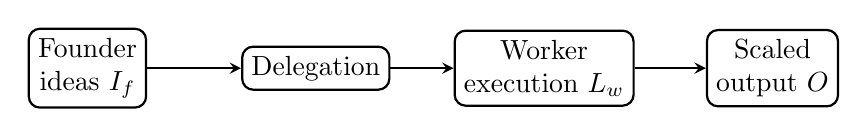
\begin{tikzpicture}[>=stealth, thick, node distance=2.9cm]
\node[draw, rounded corners, align=center] (ideas) {Founder\\ideas \(I_f\)};
\node[draw, rounded corners, right of=ideas, align=center] (delegation) {Delegation};
\node[draw, rounded corners, right of=delegation, align=center] (labor) {Worker\\execution \(L_w\)};
\node[draw, rounded corners, right of=labor, align=center] (output) {Scaled\\output \(O\)};
\draw[->] (ideas) -- (delegation);
\draw[->] (delegation) -- (labor);
\draw[->] (labor) -- (output);
\end{tikzpicture}
\end{figure}

This is the lecture's most explicit model of leverage. It is also where the rhetoric becomes more extreme. The interviewee invokes the language of workers and free thinkers, and even brings in the Rockefeller story about education producing workers rather than independent minds. That historical framing should be read as part of the speaker's own explanation, not as an independently established theorem. What matters structurally is the hierarchy he is trying to describe: idea generation at the top, delegated execution beneath it.

The lecture then sharpens the point by adding a hiring rule. The founder need not be the smartest person in the room. The speaker names employees with Yale, Stanford, and Harvard backgrounds. So the argument is not anti-education in any simple sense. It is an argument that the entrepreneur's task is to assemble intelligence and direct it, not to impersonate it alone.

The next heuristic, though rough, matters because the host chooses to freeze it in the recap:
\begin{equation}
\text{Success bottleneck} \sim 0.8\,M + 0.2\,K,
\end{equation}
where \(M\) is mindset and \(K\) is skill set.

We should not pretend this is an empirical decomposition. It is a speaker's rule of thumb. But the lecture attaches a precise meaning to it. Mindset is not mere cheerfulness. It is the capacity to steward, hold, and multiply money. In that sense, the claim that most people would lose a million-dollar windfall within six months is not meant as insult but as diagnosis: without stewardship, capital dissipates.

The host understands that the audience needs a compression here, and he gives one. He restates the lesson as plainly as possible: the number one thing keeping people broke is mindset. That recap is not ornamental. It is how the lecture seals the first mechanism before moving us to a more difficult marina and a different kind of answer.

\section{Second Marina: Older Wealth and the Difference Between Utility and Display}

The next movement is not only geographical but tonal. Access becomes harder. The host must get through a gate, persuade a stranger, and accept an interview on the stranger's terms. This change of setting matters because it also changes the shape of the answer.

Rick, the older owner, speaks less like a scaler and more like someone who has lived through many industries: clubs, jewelry, a gambling ship, a film studio. The host then asks the right question for this moment: if one could go back and advise one's younger self, what would one say?

The answer comes through a pair of functional equivalences:
\begin{align}
\text{Timekeeping}(\text{Timex}) &= \text{Timekeeping}(\text{Rolex}),\\
\text{Transport}_{A\to B}(\text{Volkswagen}) &= \text{Transport}_{A\to B}(\text{Rolls Royce}).
\end{align}

These are not equalities of cost or prestige. They are equalities of core service. Their function inside the lecture is corrective. We began from spectacle, and now the lecture forces us to distinguish function from display. A Rolex may signify something socially that a Timex does not; but if we ask what problem is being solved, both solve the same problem. Likewise for the car.

\subsection{Question \& Answer}

\paragraph{Question.}
If money buys status, what actually matters?

\paragraph{Answer.}
Rick's answer is that money is not the deepest variable. What matters is the way one treats life, oneself, and other people. What matters is what one learns at bottom. What matters is self-knowledge. In the lecture's own rhythm, this is a deliberate slowing down. We are not permitted to rush from the sight of luxury to a theory that confuses symbol with substance.

The same interview also corrects the first entrepreneur from another direction. Education, he says, might have let him go farther earlier; yet a degree is not presented as mechanically necessary for success. Education belongs, in this frame, to the improvement of decisions, not to the guarantee of reward.

When the host recaps this interview, he does something important: he does not merely repeat the sayings. He turns them into advice against envy. Do not be preoccupied by what others have; remember that your own path has its own time scale and its own sacrifices. The lecture thus uses the second interview not to abandon money, but to put money back into proportion.

\section{Another Voice: Risk, Decision, and the Unteachable Denominator}

The next interview is rougher in the transcript than the earlier ones, but several points are stable enough to preserve. The speaker reports a very large year, says he became a millionaire at twenty-four, says education gives one better tools for decision, and then sharpens the common trait among successful operators to one word: risk.

\begin{equation}
\text{no risk} \Rightarrow \text{no reward}.
\end{equation}

This is the lecture's cleanest statement of the risk-reward principle. Yet even here risk is not the final denominator. The host presses once more: how does one find the self-belief to take those risks? The answer is more severe than the earlier mindset language. According to this speaker, belief is not something one simply receives from outside instruction. It cannot be taught in the ordinary way.

\subsection{Question \& Answer}

\paragraph{Question.}
Can self-belief be taught, or is it a prerequisite?

\paragraph{Answer.}
The lecture's answer here leans toward prerequisite. Education may improve judgment. Skills may be learned. But the decisive internal permission to make the leap is treated as irreducible. The host's recap makes the point more memorable: what drove this speaker was not a single special trick, nor an external rescuer, but an unwavering belief that success would be achieved.

This is why the section cannot be reduced to generic encouragement. The lecture is trying to isolate a hidden variable that survives across different biographies. The first interview called it mindset; this one calls it self-belief. The words are not identical, but the structure is close enough that the host can use the new interview to reinforce the old result.

\section{Return to the Yacht: Hunger, Pillars, and Confidence as an Update Rule}

By the time we reach the final substantive interview, the lecture has accumulated enough partial answers that it can begin to synthesize. We return, fittingly, to a health-care entrepreneur on a yacht, which gives the chapter a kind of circular closure. The visual question from the beginning is now revisited with a fuller internal account.

The first answer in this final interview is about common traits. What do highly successful people share? Hunger. Not mere fantasy, not mere vocabulary, but hunger combined with execution. The speaker emphasizes that such people do not stop scheming, and more importantly, they act on what they scheme.

But as before, the lecture refuses to let a hard-sounding word be the last one. Hunger is not all. The speaker turns next to reading, scripture, faith, wife, and long-standing friends. When the path becomes rocky, the practical question is no longer how ambitious we are. It is what we can hold on to.

We can record the named support structure as
\begin{equation}
\mathcal{P}=\{\text{faith},\ \text{marriage},\ \text{long-term friends}\}.
\end{equation}

This is not lecture notation. It is only a compact way of preserving the list. What matters is that the lecture now places stability outside the isolated self. Endurance is scaffolded.

\subsection{Question \& Answer}

\paragraph{Question.}
What do we hang on to when scaling gets rocky?

\paragraph{Answer.}
The answer is not abstract spirituality alone, nor self-reliance alone. It is a small, durable support system: faith, spouse, and old friends. The lecture is careful here. It does not deny the importance of internal will, but it insists that internal steadiness is held up by pillars that are relational and spiritual as well as personal.

The closing exhortation then turns these supports back into process. Confidence is not treated as a mysterious gift. It is built. The lecture's final logic can be written in compressed form as
\begin{equation}
G_d \to C \to G_{\text{larger}},
\end{equation}
where \(G_d\) denotes completed daily goals, \(C\) denotes accumulated confidence, and \(G_{\text{larger}}\) denotes larger goals that become attackable only after that confidence has been built.

The derivation is straightforward and worth recording explicitly:
\begin{enumerate}
\item We make daily promises to ourselves.
\item We keep those promises.
\item Kept promises accumulate into completed daily goals.
\item Completed daily goals accumulate into confidence.
\item That confidence makes larger goals psychologically and practically accessible.
\end{enumerate}

This is the most process-like statement in the entire lecture. It is also the best answer to a possible misunderstanding. The chapter has spoken a good deal about self-belief, but it does not end by saying: simply believe. It ends by saying: belief is reinforced by disciplined repetition. Confidence is the visible remainder of promises kept.

The host's final spoken response to this interview confirms the intended reading. He hears in the answer not vague motivation but something concrete enough to say, with admiration, that such material is not taught in school.

\section{Summary}

The lecture begins with a yacht and ends with a structure. First the host gives us a teaser of large numbers; then he frames Miami as a city in which visible wealth may be studied rather than merely envied. The first stable case gives us the strongest data and the clearest mechanism: founder time is the scarce asset, and eight figures require delegation rather than heroic self-exhaustion. The second voice slows us down and distinguishes utility from display. The third sharpens the role of risk and self-belief. The final voice gathers the whole chapter into hunger, faith, circle, and the discipline by which confidence is accumulated.

So the chapter's mathematics is simple, but it is not superficial. We have a city-scale number, a business ledger, an implied margin, a bottleneck variable, a leverage diagram, a functional equivalence, a risk law, and a small update rule for confidence. None of this is blackboard mathematics in the usual sense. Yet it is exactly the kind of structure the lecture keeps reaching for: underneath the visible symbol of wealth there is a sequence of constraints, choices, and supports. That is the real object we have been tracking from the start.